\documentclass{article}
\usepackage[utf8]{inputenc}
\usepackage[english]{babel}
\usepackage[letterpaper, portrait, margin=1in]{geometry}
\usepackage[authoryear,round]{natbib}
\usepackage[colorlinks=true,citecolor=teal, linkcolor=Periwinkle,urlcolor=Periwinkle]{hyperref}
\usepackage[dvipsnames]{xcolor}
\usepackage{graphicx}
\usepackage{amsmath}

\title{Perceptual Losses for Real-Time Style~Transfer and~Super-Resolution}
\author{Iantsa~Provost, Lilian~Rebiere, Bastien~Soucasse, and~Alexey~Zhukov}
\date{January~5, 2022}

\linespread{1.15}
\bibliographystyle{abbrvnat}

\begin{document}

% Title Page
{
    \begin{titlepage}
        \begin{center}
            \vspace*{1.5cm}

            \Large

            \textbf{Perceptual Losses for Real-Time Style~Transfer and~Super-Resolution}

            \vspace{.5cm}

            \vspace{1.5cm}

            \large

            \textbf{Iantsa~Provost, Lilian~Rebiere-Pouyade, Bastien~Soucasse, and~Alexey~Zhukov}

            \vfill

            \normalsize

            Presented as part of the\\
            \textit{AMIP}\\
            course unit.

            \vspace{1.5cm}

            
\includegraphics[width=.5\textwidth]{images/college-logo.jpg}

            Computer~Science~Master's~Degree in~Image~and~Sound\\
            Université~de~Bordeaux,~France\\
            January~5,~2022
        \end{center}
    \end{titlepage}
    \newpage
    \setcounter{page}{2}
}

% Table of Contents
{
    \hypersetup{linkcolor=black}
    \tableofcontents
    \newpage
}

% Introduction
{
    \section{Introduction}
    \label{sec:introduction}

    \cite{sr} introduced neural network models for style transfer and super-resolution, based on the convolutional neural networks (CNNs) for image transformation introduced by \cite{image-transform-network}.

    The image transformation models take an image as input and produce a transformed version of this image. They are trained by minimizing a loss function between this produced image and a target image.

    The key upgrade is the use of perceptual loss functions for a feature-wise similarity score---instead of pixel-wise---when checking the similarity between the generated image and the target image. This technique focuses on the similarity between high-level feature components of the images---instead of their pixels---and therefore maintains the perceptual quality of the generated image.

    \bigskip

    We propose an implementation of the super-resolution model by \cite{sr}. Super-resolution models are used to generate high-resolution (HR) images from low-resolution (LR) versions. These methods apply to image processing, computer vision, and medical imaging.

    To train the model, we use a dataset of HR images and generate the LR version of these images. We use the LR images as input for the model, and HR versions as the ground-truth target.

    \bigskip

    In this report, we present and explain the method used in the model, describe any implementation difficulties that we encountered, and analyze the qualitative and quantitative results of the experiments. We also discuss the energy consumption used during the project and consider other possible impacts. Finally, we suggest possible extensions and future directions for this work.
}

% Method
{
    \section{Method}
    \label{sec:method}

    \begin{figure*}[ht]
        \centering
        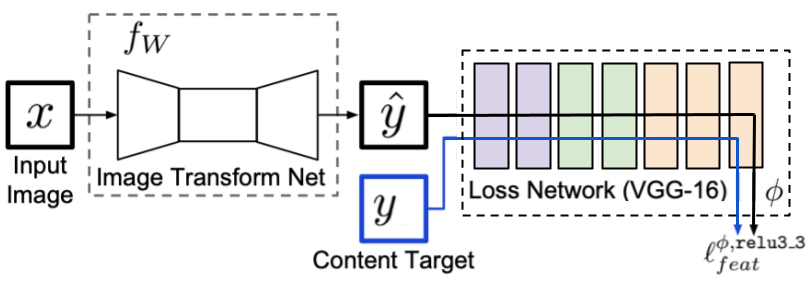
\includegraphics[width=\textwidth]{images/model.png}
        \caption{Overview of the architecture of the model proposed by \cite{sr}, focusing on super-resolution.}
        \label{fig:model}
    \end{figure*}

    The proposed model illustrated in Figure~\ref{fig:model} consists of two components: the image transformation network $f_W$ and a loss network $\phi$. Given a low-resolution input image $x$, it generates an output image that is expected to be similar to the ground truth high-resolution image $y$.

    The image transformation network is a deep residual convolutional neural network with a set of weights parameter denoted $W$. From input images $x$, it provides output images $\hat y$.

    The loss network defines a feature reconstruction loss $l^\phi_{feat}$. It delineates several feature reconstruction loss functions $l^{\phi, i}_{feat}(\hat y, y_i)$ that each measure the difference in content between output image $\hat y$ and content target images $y_i$. Here, $i$ denotes the layer.
    % I didn't precise "yc" (which makes the difference with "ys" for style transfer) because we only measure the content difference in our case. It could be modified if you think it's necessary.
    Furthermore, \cite{sr} drew inspiration from several papers such as the one by \cite{gatys} in order to make the most of their feature reconstruction loss. The principle is to use a network pre-trained for image classification as a loss network. This way, the beforehand learning of the perceptual and semantic information will facilitate the measure computation of the feature reconstruction loss.

    \bigskip

    Gathering both components, the image transformation network adjusts its weights $W$ by minimizing the combination of those loss functions, using stochastic gradient descent (Equation~\ref{eq:sgd}). Note that the formula given in the paper \citep{sr} mentions a “weighted combination of loss functions” but does not provide more information about the aforementioned weights. As a consequence, we decided to set them all to 1.
    % It only uses a small batch of data to compute the update step at each iteration instead of the average of the gradients in classic gradient descent.

    \begin{equation}
        W^* = \text{argmin}_W \textbf{E}_{x,y_i} \biggl[ \sum_{i=0} l^{\phi, i}_{feat}(f_W(x), y_i) \biggr]
        \label{eq:sgd}
    \end{equation}

    \subsection{Image Transfomation Network}
    \label{subsec:image-transformation-network-method}

    As mentioned previously, the image transformation network is a deep residual convolutional neural network. That is, it includes residual blocks that prevent vanishing gradient issues---when the gradients of the parameters become very small, hindering the ability of the network to learn and improve.

    Residual blocks in the model are defined using the architecture design of \cite{rb}, with the exception of the deletion of the last activation ReLU. 
      
     This network takes as input a low resolution image of shape $3 \times 288/f \times 288/f$, and resulting an output image of shape $3 \times 288 \times 288$, which is a high-resolution version of the input image.

    \subsection{Loss Network}
    \label{subsec:loss-network-method}

    What propose \cite{sr} is to try and make the images have similar feature representations, instead of forcing a pixel-per-pixel match. To do so and to make it more performant, the loss network is here defined as a pre-trained network for image classification. More specifically, they use the 16-layer VGG network \citep{vgg} pre-trained on the ImageNet dataset \citep{image-net}.

    Now to compute the feature reconstruction loss $l^{\phi, i}_{feat}$ in Equation~\ref{eq:sgd} between the output $\hat y$ and the content target $y$ at a layer $i$, we use the mean square Euclidean distance (Equation~\ref{eq:loss-formula}).

    \begin{equation}
        l^{\phi, i}_{feat}(f_W(x), y_i) = \frac{1}{C_i H_i W_i} \lVert \phi_i (\hat y) - \phi_i (y) \rVert_2^2
        \label{eq:loss-formula}
    \end{equation}

    Note that $C_i$, $H_i$, and $W_i$ are respectively the number of channels, height, and width of the input image. And, $\phi_i (x)$ is the feature representation of $x$ at layer $i$ (here, $x$ does not mean the input image, but an arbitrary image).
}

% Implementation
{
    \section{Implementation}
    \label{sec:implementation}

    \subsection{Image Transformation Network}
    \label{subsec:image-transformation-network-implementation}

    First of all, the super-resolution model was implemented following the original paper \citep{sr}. The model is based on the image transformation model class defined by \cite{image-transform-network}.

    \bigskip

    Before all, a simple upsampling layer has been added to create a larger image from the input one according to the upsampling factor of the architecture—it is either 4 or 8.

    First of all, the model is then constructed with an input convolutional layer with a kernel size of 9, followed by four successive residual blocks \citep{residual}.
  

    Each residual block is composed of two convolution layers with a kernel size of 3. The first one is activated with the ReLU function. Finally, the block's initial input (before the convolutional layers) is added to the output of the block---this is the residual part.

    After that, just before the output convolutional layer, with a kernel of size 9, there are other convolutional layers. The number of these convolutional layers, with a kernel of size 4 and, in our case a stride of 1, depends on the upsampling factor. Indeed,  two layers are used if the upsampling factor is set to 4, whereas three layers are set up if scaling factor is set to 8.

    Finally, on both layers of the network, each convolutional layers have the same number of filters with is 64, followed by spatial batch normalization and a ReLU non-linearity, excepted on the output layer, without batch normalization, and which uses a scaled tanh to respect the pixels range.

    \bigskip

    […]

    \subsection{Loss Network}
    \label{subsec:loss-network-implementation}

    As previously mentioned, the loss network is based on VGG-16 \citep{vgg}. We use pre-trained weights on ImageNet \citep{image-net} automatically downloaded from the PyTorch website. This VGG-16 instance is frozen and set to evaluation mode.

    \bigskip

    When called with generated and output images, the model retrieves the features from the two images. It can then compute the sum of the mean squared Euclidian distances (MSEs). This sum is the actual loss between the two images, used for backpropagation in the image transformation model.

    \subsection{Suggested Optimization}
    \label{subsec:suggested-optimization}

    The goal of using the feature loss instead of the pixel-wise MSE loss was to compute the perceptual similarity score instead of the difference between each pixel, as previously established. But we wondered what could be the result when combining such a perceptual loss and the original pixel loss, by summing the two of them. We implemented a simple option to activate this potential optimization. The results will be put in comparison in Section~\ref{sec:experiments}.
}

% Experiments
{
    \section{Experiments}
    \label{sec:experiments}

    \subsection{Setup}
    \label{subsec:setup}

    In order to conduct experiments, we first need a dataset to train our model. \cite{sr} used the Microsoft Common Objects in Context (MS-COCO) dataset \citep{mscoco} for training, but due to its large size and the associated training time, we had to find a more adequate dataset.

    As an alternative, we chose DIV2K, a dataset introduced by \cite{div2k_ds} in the technical report \textit{2017 IEEE Conference on Computer Vision and Pattern Recognition Workshops (CVPRW)}. DIV2K is a widely-used dataset for super-resolution tasks containing 1000 pairs of low-resolution (LR) and high-resolution (HR) images. Compared to the MS-COCO dataset, it has a reasonable size, making it more feasible for use in this study. More specifically, we only used the HR images dedicated to training: 800 images of variable sizes. An extract is visualizable in Figure~\ref{fig:div2k-train-og}.

    \begin{figure*}[ht]
        \centering
        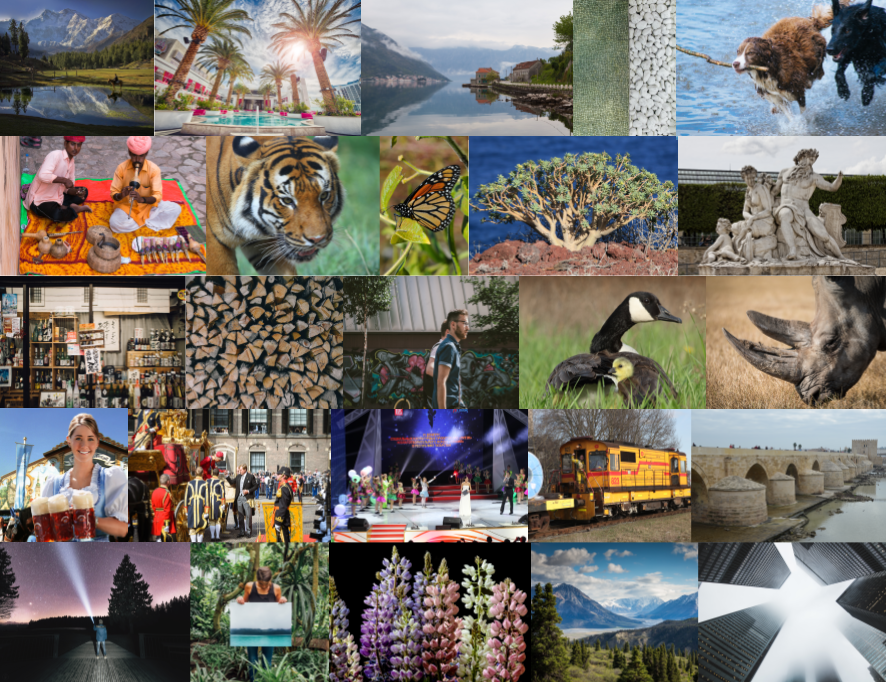
\includegraphics[width=\textwidth]{images/DIV2K_HR.png}
        \caption{Visualization of 25 DIV2K HR train images.}
        \label{fig:div2k-train-og}
    \end{figure*}

    \bigskip

    As the model needs a specific type of training data, we did not use the LR images of DIV2K. Instead, we decided to process directly the HR images to create our custom HR-LR pairs of images.
    % Furthermore, it allows the storage of fewer images.

    To do so, the original HR images are cropped to $288 \times 288$ to create the HR patches. Then they are pre-processed according to the methods described in the paper \citep{sr}, to create the corresponding LR patches. It consists in blurring the cropped image with a Gaussian kernel of width $\sigma = 1.0$, and downsampling the result with bicubic interpolation.

    Now that the dataset is pre-processed (see extract in Figure~\ref{fig:div2k-train-pair}), the model and its dataset are ready to be used for training.

    \begin{figure*}[p]
        \centering
        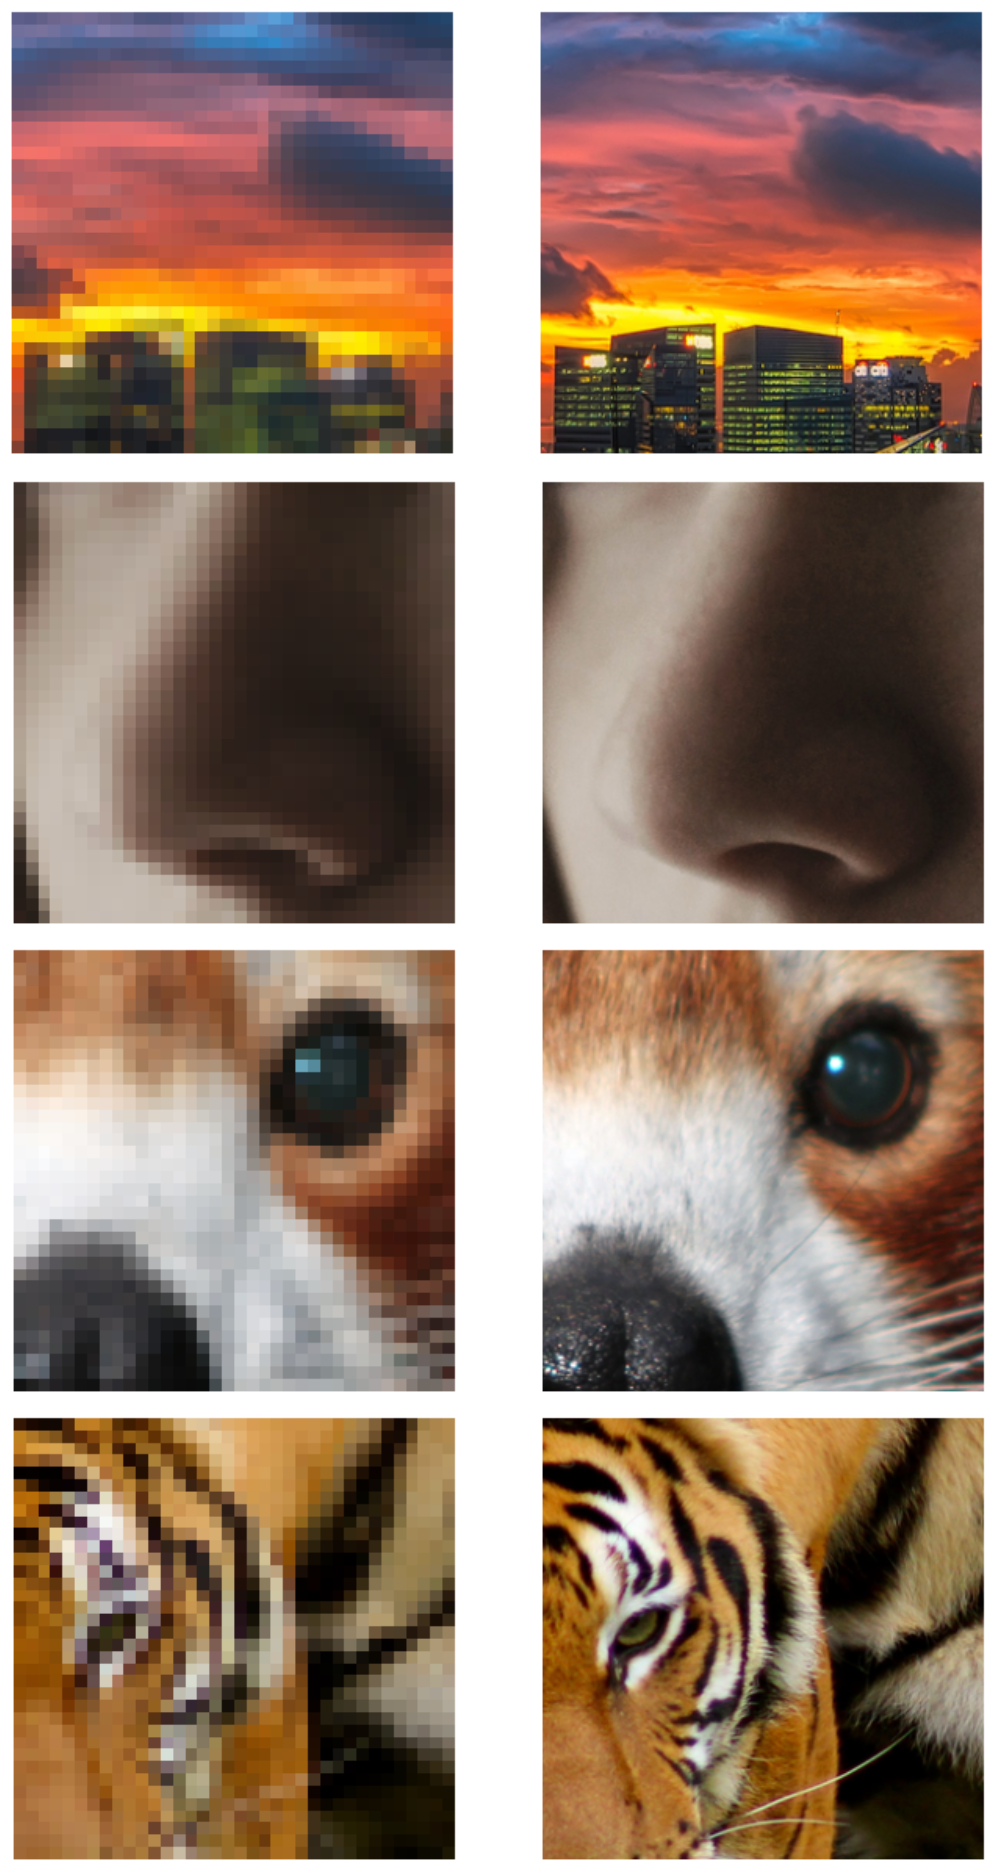
\includegraphics[height=0.9\textheight]{images/DIV2K_HRLR.png}
        \caption{Visualization of 4 pairs of DIV2K HR train images (right) and their LR corresponding images (left), that underwent our pre-processing.}
        \label{fig:div2k-train-pair}
    \end{figure*}

    \subsection{Training}
    \label{subsec:training}

    To train our model, we have defined some hyper parameters according to the original paper. Indeed, we use the Adam optimizer, defined the learning rate to $1 \times 10^{-3}$ and also a batch size of 4.
    Concerning the loss function, it is determined as detailed in the section ~\ref{subsec:loss-network-implementation}.
    
    Finally, we experimented different values to determine, in our opinion, what is the best number of epochs to get the best results in the test phase. In our case, and in view of the various results, we have thus defined the number of epochs as 5.

    \subsection{Testing}
    \label{subsec:testing}

    […]
}

% Environmental Impact
{
    \section{Environmental Impact}
    \label{sec:env-impact}

    […]
}

% Conclusion
{
    \section{Conclusion}
    \label{sec:conclusion}

    […]
}

% References
{
    \bibliography{references}
}

\end{document}
